% Judul dokumen
\title{Buku Tugas Akhir ITS}
\author{Musk, Elon Reeve}

% Pengaturan ukuran teks dan bentuk halaman dua sisi
\documentclass[12pt,twoside]{report}

% Pengaturan ukuran halaman dan margin
\usepackage[a4paper,top=30mm,left=30mm,right=20mm,bottom=25mm]{geometry}

% Pengaturan ukuran spasi
\usepackage[singlespacing]{setspace}

% Pengaturan detail pada file PDF
\usepackage[pdfauthor={\@author},bookmarksnumbered,pdfborder={0 0 0}]{hyperref}

% Pengaturan jenis karakter
\usepackage[utf8]{inputenc}

% Pengaturan pewarnaan
\usepackage[table,xcdraw]{xcolor}

% Pengaturan kutipan artikel
\usepackage[style=apa, backend=biber]{biblatex}

% Package lainnya
\usepackage{changepage}
\usepackage{enumitem}
\usepackage{eso-pic}
\usepackage{txfonts} % Font times
\usepackage{etoolbox}
\usepackage{graphicx}
\usepackage{lipsum}
\usepackage{longtable}
\usepackage{tabularx}
\usepackage{wrapfig}
\usepackage{float}
\usepackage[T1]{fontenc}

% Definisi untuk "Hati ini sengaja dikosongkan"
\patchcmd{\cleardoublepage}{\hbox{}}{
  \thispagestyle{empty}
  \vspace*{\fill}
  \begin{center}\textit{[Halaman ini sengaja dikosongkan]}\end{center}
  \vfill}{}{}

% Pengaturan penomoran halaman
\usepackage{fancyhdr}
\fancyhf{}
\renewcommand{\headrulewidth}{0pt}
\pagestyle{fancy}
\fancyfoot[LE,RO]{\thepage}
\patchcmd{\chapter}{plain}{fancy}{}{}
\patchcmd{\chapter}{empty}{plain}{}{}

% Command untuk bulan
\newcommand{\MONTH}{%
  \ifcase\the\month
  \or Januari% 1
  \or Februari% 2
  \or Maret% 3
  \or April% 4
  \or Mei% 5
  \or Juni% 6
  \or Juli% 7
  \or Agustus% 8
  \or September% 9
  \or Oktober% 10
  \or November% 11
  \or Desember% 12
  \fi}
\newcommand{\ENGMONTH}{%
  \ifcase\the\month
  \or January% 1
  \or February% 2
  \or March% 3
  \or April% 4
  \or May% 5
  \or June% 6
  \or July% 7
  \or August% 8
  \or September% 9
  \or October% 10
  \or November% 11
  \or December% 12
  \fi}

% Pengaturan format judul bab
\usepackage{titlesec}
\titleformat{\chapter}[display]{\bfseries\Large}{BAB \centering\Roman{chapter}}{0ex}{\vspace{0ex}\centering}
\titleformat{\section}{\bfseries\large}{\MakeUppercase{\thesection}}{1ex}{\vspace{1ex}}
\titleformat{\subsection}{\bfseries\large}{\MakeUppercase{\thesubsection}}{1ex}{}
\titleformat{\subsubsection}{\bfseries\large}{\MakeUppercase{\thesubsubsection}}{1ex}{}
\titlespacing{\chapter}{0ex}{0ex}{4ex}
\titlespacing{\section}{0ex}{1ex}{0ex}
\titlespacing{\subsection}{0ex}{0.5ex}{0ex}
\titlespacing{\subsubsection}{0ex}{0.5ex}{0ex}

% Atur variabel berikut sesuai namanya

% nama
\newcommand{\name}{I Gusti Made Arisudana}
\newcommand{\authorname}{Arisudana, I Gusti Made}
\newcommand{\nickname}{Arisudana}
\newcommand{\advisor}{Retno Aulia Vinarti, S.Kom., M.Kom., Ph.D.}
\newcommand{\coadvisor}{Izzat Aulia Akbar, S.Kom., M.Eng., Ph.D.}
\newcommand{\examinerone}{Amalia Utamima, S.Kom., MBA., Ph.D.}
\newcommand{\examinertwo}{Renny Pradina Kusumawardani, S.T., M.T.}
\newcommand{\examinerthree}{Alan Turing, ST., MT}
\newcommand{\headofdepartment}{Prof. Albus Percival Wulfric Brian Dumbledore, S.T., M.T}

% identitas
\newcommand{\nrp}{5026211188}
\newcommand{\advisornip}{1988201812010 }
\newcommand{\coadvisornip}{1991202011006}
\newcommand{\examineronenip}{18560710 194301 1 001}
\newcommand{\examinertwonip}{18560710 194301 1 001}
\newcommand{\examinerthreenip}{18560710 194301 1 001}
\newcommand{\headofdepartmentnip}{18810313 196901 1 001}

% judul
\newcommand{\tatitle}{SISTEM REKOMENDASI PROPERTI BERBASIS \emph{HYBRID FILTERING} DAN \emph{PROFILE MATCHING}}
\newcommand{\engtatitle}{\emph{PROPERTY RECOMMENDATION SYSTEMS BASED ON HYBRID FILTERING AND PROFILE MATCHING}}

% tempat
\newcommand{\place}{Surabaya}

% jurusan
\newcommand{\studyprogram}{Sistem Informasi}
\newcommand{\engstudyprogram}{Information Systems}

% fakultas
\newcommand{\faculty}{Teknologi Elektro dan Informatika Cerdas}
\newcommand{\engfaculty}{Intelligent Electrical and Informatics Technology}

% singkatan fakultas
\newcommand{\facultyshort}{FTEIC}
\newcommand{\engfacultyshort}{ELECTICS}

% departemen
\newcommand{\department}{Sistem Informasi}
\newcommand{\engdepartment}{Information Systems}

% kode mata kuliah
\newcommand{\coursecode}{ES234849}


% Tambahkan format tanda hubung yang benar di sini
\hyphenation{
  ro-ket
  me-ngem-bang-kan
  per-hi-tu-ngan
  tek-no-lo-gi
  me-la-ku-kan
  ber-so-si-al-i-sa-si
}

% Menambahkan resource daftar pustaka
\addbibresource{pustaka/pustaka.bib}

% Pengaturan format potongan kode
\usepackage{listings}
\definecolor{comment}{RGB}{0,128,0}
\definecolor{string}{RGB}{255,0,0}
\definecolor{keyword}{RGB}{0,0,255}
\lstdefinestyle{codestyle}{
  commentstyle=\color{comment},
  stringstyle=\color{string},
  keywordstyle=\color{keyword},
  basicstyle=\footnotesize\ttfamily,
  numbers=left,
  numberstyle=\tiny,
  numbersep=5pt,
  frame=lines,
  breaklines=true,
  prebreak=\raisebox{0ex}[0ex][0ex]{\ensuremath{\hookleftarrow}},
  showstringspaces=false,
  upquote=true,
  tabsize=2,
}
\lstset{style=codestyle}

% Isi keseluruhan dokumen
\begin{document}

% Sampul luar Bahasa Indonesia
\newcommand\covercontents{sampul/konten-id.tex}
\AddToShipoutPictureBG*{
  \AtPageLowerLeft{
    % Ubah nilai berikut jika posisi horizontal background tidak sesuai
    \hspace{-3.25mm}

    % Ubah nilai berikut jika posisi vertikal background tidak sesuai
    \raisebox{0mm}{
      
\includegraphics[width=\paperwidth,height=\paperheight]{sampul/gambar/sampul-luar.png}
    }
  }
}

% Menyembunyikan nomor halaman
\thispagestyle{empty}

% Pengaturan margin untuk menyesuaikan konten sampul
\newgeometry{
  top=55mm,
  left=30mm,
  right=20mm,
  bottom=20mm
}

\begin{flushleft}

  % Pemilihan font sans serif
  \sffamily

  % Pemilihan warna font putih
  \color{white}

  % Pemilihan font bold
  \fontseries{bx}
  \selectfont
  \begin{spacing}{1.5}
    \input{\covercontents}
  \end{spacing}

\end{flushleft}

\restoregeometry


% Atur ulang penomoran halaman
\setcounter{page}{1}

% Sampul dalam Bahasa Indonesia
\renewcommand\covercontents{sampul/konten-id.tex}
\AddToShipoutPictureBG*{
  \AtPageLowerLeft{
    % Ubah nilai berikut jika posisi horizontal background tidak sesuai
    \hspace{-4mm}

    % Ubah nilai berikut jika posisi vertikal background tidak sesuai
    \raisebox{0mm}{
      
\includegraphics[width=\paperwidth,height=\paperheight]{sampul/gambar/sampul-luar-tipis.png}
    }
  }
}

% Menyembunyikan nomor halaman
\thispagestyle{empty}

% Pengaturan margin untuk menyesuaikan konten sampul
\newgeometry{
  top=65mm,
  left=30mm,
  right=30mm,
  bottom=20mm
}

\begin{flushleft}

  % Pemilihan font sans serif
  \sffamily

  % Pemilihan font bold
  \fontseries{bx}
  \selectfont
  \begin{spacing}{1.5}
    \input{\covercontents}
  \end{spacing}

\end{flushleft}

\restoregeometry

\clearpage
\cleardoublepage

% Sampul dalam Bahasa Inggris
\renewcommand\covercontents{sampul/konten-en.tex}
\AddToShipoutPictureBG*{
  \AtPageLowerLeft{
    % Ubah nilai berikut jika posisi horizontal background tidak sesuai
    \hspace{-4mm}

    % Ubah nilai berikut jika posisi vertikal background tidak sesuai
    \raisebox{0mm}{
      
\includegraphics[width=\paperwidth,height=\paperheight]{sampul/gambar/sampul-luar-tipis.png}
    }
  }
}

% Menyembunyikan nomor halaman
\thispagestyle{empty}

% Pengaturan margin untuk menyesuaikan konten sampul
\newgeometry{
  top=65mm,
  left=30mm,
  right=30mm,
  bottom=20mm
}

\begin{flushleft}

  % Pemilihan font sans serif
  \sffamily

  % Pemilihan font bold
  \fontseries{bx}
  \selectfont
  \begin{spacing}{1.5}
    \input{\covercontents}
  \end{spacing}

\end{flushleft}

\restoregeometry

\cleardoublepage

% Label tabel dan gambar dalam bahasa indonesia
\renewcommand{\figurename}{Gambar}
\renewcommand{\tablename}{Tabel}

% Pengaturan ukuran indentasi paragraf
\setlength{\parindent}{2em}

% Pengaturan ukuran spasi paragraf
\setlength{\parskip}{1ex}

% Lembar pengesahan
\begin{center}
  \large
  \textbf{LEMBAR PENGESAHAN}
\end{center}

% Menyembunyikan nomor halaman
\thispagestyle{empty}

\begin{center}
  \textbf{\tatitle{}}
\end{center}

\begingroup
% Pemilihan font ukuran small
\small

\begin{center}
  \textbf{TUGAS AKHIR}
  \\Diajukan untuk memenuhi salah satu syarat \\
  memperoleh gelar Sarjana pada \\
  Program Studi S-1 \studyprogram{} \\
  Departemen \department{} \\
  Fakultas \faculty{} \\
  Institut Teknologi Sepuluh Nopember
\end{center}

\begin{center}
  Oleh: \textbf{\name{}}
  \\NRP. \nrp{}
\end{center}

\begin{center}
  Disetujui oleh Tim Penguji Tugas Akhir:
\end{center}

\begingroup
% Menghilangkan padding
\setlength{\tabcolsep}{0pt}

\noindent
\begin{tabularx}{\textwidth}{X l}
  \advisor{}               & Pembimbing                        \\
                           &                                     \\
                           &                                     \\
  \coadvisor{}             & Ko-Pembimbing                     \\
                           &                                     \\
                           &                                     \\
  \examinerone{}.          & Penguji I                         \\
                           &                                     \\
                           &                                     \\
  \examinertwo{}.          & Penguji II                        \\
                           &                                     \\
                           &                                     \\

\end{tabularx}
\endgroup

\begin{center}
  \textbf{\MakeUppercase{\place{}}\\\MONTH{}, \the\year{}}
\end{center}
\endgroup

\cleardoublepage
\begin{center}
  \large
  \textbf{APPROVAL SHEET}
\end{center}

% Menyembunyikan nomor halaman
\thispagestyle{empty}

\begin{center}
  \textbf{\engtatitle{}}
\end{center}

\begingroup
% Pemilihan font ukuran small
\small

\begin{center}
  \textbf{FINAL PROJECT}
  \\Submitted to fulfill one of the requirements \\
  for obtaining a degree Bachelor of Engineering at \\
  Undergraduate Study Program of \engstudyprogram{} \\
  Department of \engdepartment{} \\
  Faculty of \engfaculty{} \\
  Sepuluh Nopember Institute of Technology
\end{center}

\begin{center}
  By: \textbf{\name{}}
  \\NRP. \nrp{}
\end{center}

\begin{center}
  Approved by Final Project Examiner Team:
\end{center}

\begingroup
% Menghilangkan padding
\setlength{\tabcolsep}{0pt}

\noindent
\begin{tabularx}{\textwidth}{X l}
  \advisor{}               & (Advisor I)                         \\
  NIP: \advisornip{}       &                                     \\
                           & ................................... \\
                           &                                     \\
                           &                                     \\
  \coadvisor{}             & (Co-Advisor II)                     \\
  NIP: \coadvisornip{}     &                                     \\
                           & ................................... \\
                           &                                     \\
                           &                                     \\
  \examinerone{}.          & (Examiner I)                        \\
  NIP: \examineronenip{}   &                                     \\
                           & ................................... \\
                           &                                     \\
                           &                                     \\
  \examinertwo{}.          & (Examiner II)                       \\
  NIP: \examinertwonip{}   &                                     \\
                           & ................................... \\
                           &                                     \\
                           &                                     \\
  \examinerthree{}.        & (Examiner III)                      \\
  NIP: \examinerthreenip{} &                                     \\
                           & ................................... \\
\end{tabularx}
\endgroup


\begin{center}
  Acknowledged, \\
  Head of \engdepartment{} Department \engfacultyshort{} - ITS \\

  \vspace{8ex}

  \underline{\headofdepartment{}.} \\
  NIP. \headofdepartmentnip{}
\end{center}

\begin{center}
  \textbf{\MakeUppercase{\place{}}\\\ENGMONTH{}, \the\year{}}
\end{center}
\endgroup

\cleardoublepage

% Pernyataan keaslian
\begin{center}
  \large
  \textbf{PERNYATAAN ORISINALITAS}
\end{center}

% Menyembunyikan nomor halaman
\thispagestyle{empty}

\vspace{2ex}

% Ubah paragraf-paragraf berikut sesuai dengan yang ingin diisi pada pernyataan keaslian

\noindent Yang bertanda tangan dibawah ini:

\noindent\begin{tabularx}{\textwidth}{l l X}
                         &   &                            \\
  Nama Mahasiswa / NRP   & : & \name{} / \nrp{}           \\
  Departemen             & : & \department{}              \\
  Dosen Pembimbing / NIP & : & \advisor{} / \advisornip{} \\
                         &   &                            \\
\end{tabularx}

Dengan ini menyatakan bahwa Tugas Akhir dengan judul "\tatitle{}" adalah hasil karya sendiri, berfsifat orisinal, dan ditulis dengan mengikuti kaidah penulisan ilmiah.

Bilamana di kemudian hari ditemukan ketidaksesuaian dengan pernyataan ini, maka saya bersedia menerima sanksi sesuai dengan ketentuan yang berlaku di Institut Teknologi Sepuluh Nopember.

\vspace{8ex}

\noindent\begin{tabularx}{\textwidth}{X l}
                     & \place{}, \ENGMONTH{} \the\year{} \\
                     &                                   \\
  Mengetahui         &                                   \\
  Dosen Pembimbing   & Mahasiswa                         \\
                     &                                   \\
                     &                                   \\
                     &                                   \\
                     &                                   \\
                     &                                   \\
  \advisor{}         & \name{}                           \\
  NIP. \advisornip{} & NRP. \nrp{}                       \\
\end{tabularx}

\cleardoublepage
\begin{center}
  \large
  \textbf{STATEMENT OF ORIGINALITY}
\end{center}

% Menyembunyikan nomor halaman
\thispagestyle{empty}

\vspace{2ex}

% Ubah paragraf-paragraf berikut sesuai dengan yang ingin diisi pada pernyataan keaslian

\noindent The undersigned below:

\noindent\begin{tabularx}{\textwidth}{l l X}
                        &   &                            \\
  Name of student / NRP & : & \name{} / \nrp{}           \\
  Department            & : & \engdepartment{}           \\
  Advisor / NIP         & : & \advisor{} / \advisornip{} \\
                        &   &                            \\
\end{tabularx}

Hereby declared that the Final Project with the title of "\engtatitle{}" is the result of my own work, is original, and is written by following the rules of scientific writing.

If in future there is a discrepancy with this statement, then I am willing to accept sanctions in accordance with provisions that apply at Sepuluh Nopember Institute of Technology.

\vspace{8ex}

\noindent\begin{tabularx}{\textwidth}{X l}
                     & \place{}, \ENGMONTH{} \the\year{} \\
                     &                                   \\
  Acknowledged       &                                   \\
  Advisor            & Student                           \\
                     &                                   \\
                     &                                   \\
                     &                                   \\
                     &                                   \\
                     &                                   \\
  \advisor{}         & \name{}                           \\
  NIP. \advisornip{} & NRP. \nrp{}                       \\
\end{tabularx}
\cleardoublepage

% Nomor halaman pembuka dimulai dari sini
\pagenumbering{roman}

% Abstrak Bahasa Indonesia
\begin{center}
  \large\textbf{ABSTRAK}
\end{center}

\addcontentsline{toc}{chapter}{ABSTRAK}

\vspace{2ex}

\begingroup
% Menghilangkan padding
\setlength{\tabcolsep}{0pt}

\noindent
\begin{tabularx}{\textwidth}{l >{\centering}m{2em} X}
  Nama Mahasiswa    & : & \name{}         \\

  Judul Tugas Akhir & : & \tatitle{}      \\

  Pembimbing        & : & 1. \advisor{}   \\
                    &   & 2. \coadvisor{} \\
\end{tabularx}
\endgroup

% Ubah paragraf berikut dengan abstrak dari tugas akhir
Pada penelitian ini kami mengajukan \lipsum[1]

% Ubah kata-kata berikut dengan kata kunci dari tugas akhir
Kata Kunci: Roket, \emph{Anti-gravitasi}, Energi, Angkasa.

\cleardoublepage

% Abstrak Bahasa Inggris
\begin{center}
  \large\textbf{ABSTRACT}
\end{center}

\addcontentsline{toc}{chapter}{ABSTRACT}

\vspace{2ex}

\begingroup
% Menghilangkan padding
\setlength{\tabcolsep}{0pt}

\noindent
\begin{tabularx}{\textwidth}{l >{\centering}m{3em} X}
  \emph{Name}     & : & \name{}         \\

  \emph{Title}    & : & \engtatitle{}   \\

  \emph{Advisors} & : & 1. \advisor{}   \\
                  &   & 2. \coadvisor{} \\
\end{tabularx}
\endgroup

% Ubah paragraf berikut dengan abstrak dari tugas akhir dalam Bahasa Inggris
\emph{In this research, we proposed \lipsum[1]}

% Ubah kata-kata berikut dengan kata kunci dari tugas akhir dalam Bahasa Inggris
\emph{Keywords}: \emph{Rocket}, \emph{Anti-gravity}, \emph{Energy}, \emph{Space}.

\cleardoublepage

% Kata pengantar
\begin{center}
  \Large
  \textbf{KATA PENGANTAR}
\end{center}

\addcontentsline{toc}{chapter}{KATA PENGANTAR}

\vspace{2ex}

% Ubah paragraf-paragraf berikut dengan isi dari kata pengantar

Puji dan syukur kehadirat \lipsum[1][1-5]

Penelitian ini disusun dalam rangka \lipsum[2][1-5]
Oleh karena itu, penulis mengucapkan terima kasih kepada:

\begin{enumerate}[nolistsep]

  \item Keluarga, Ibu, Bapak dan Saudara tercinta yang telah \lipsum[3][1-2]

  \item Bapak Nikola Tesla, S.T., M.T., selaku \lipsum[4][1-2]

  \item \lipsum[5][1-3]

\end{enumerate}

Akhir kata, semoga \lipsum[6][1-8]

\begin{flushright}
  \begin{tabular}[b]{c}
    \place{}, \MONTH{} \the\year{} \\
    \\
    \\
    \\
    \\
    \name{}
  \end{tabular}
\end{flushright}

\cleardoublepage

% Daftar isi
\renewcommand*\contentsname{DAFTAR ISI}
\addcontentsline{toc}{chapter}{\contentsname}
\tableofcontents
\cleardoublepage

% Daftar gambar
\renewcommand*\listfigurename{DAFTAR GAMBAR}
\addcontentsline{toc}{chapter}{\listfigurename}
\listoffigures
\cleardoublepage

% Daftar tabel
\renewcommand*\listtablename{DAFTAR TABEL}
\addcontentsline{toc}{chapter}{\listtablename}
\listoftables
\cleardoublepage

% Nomor halaman isi dimulai dari sini
\pagenumbering{arabic}

% Bab 1 pendahuluan
\chapter{PENDAHULUAN}
\label{chap:pendahuluan}

% Ubah bagian-bagian berikut dengan isi dari pendahuluan

\section{Latar Belakang}
\label{sec:latarbelakang}

Tempat tinggal merupakan salah satu kebutuhan mendasar bagi setiap individu. 
Tempat tinggal tidak hanya berfungsi sebagai sarana fisik untuk perlindungan, tetapi juga berperan dalam pemenuhan aspek psikologis dan sosial individu. 
Mengingat pentingnya peran tempat tinggal dalam kehidupan, keputusan untuk memilih properti menjadi proses yang sangat krusial. 
Sebagian besar individu jarang melakukan transaksi pembelian atau penyewaan properti sepanjang hidup mereka, sehingga setiap keputusan terkait tempat tinggal membutuhkan pertimbangan yang matang dan menyeluruh. 
Kompleksitas ini tidak hanya muncul dari tingginya nilai ekonomi properti, tetapi juga karena banyaknya faktor yang perlu diperhatikan, seperti lokasi, harga, ukuran, fasilitas, serta preferensi pribadi \parencite{Gharahighehi2021}. 
Oleh karena itu, proses pemilihan tempat tinggal sering kali melibatkan pencarian informasi yang intensif, baik secara konvensional maupun melalui platform digital.

Di era digital saat ini, penggunaan platform daring untuk mencari properti mengalami peningkatan signifikan. 
Konsumen semakin beralih ke situs web dan aplikasi untuk mengeksplorasi pilihan properti yang tersedia. 
Namun, meskipun akses informasi menjadi lebih mudah, pengguna sering menghadapi tantangan baru dalam bentuk "\emph{information overload}" atau kelebihan informasi. 
Banyaknya pilihan properti yang tersedia justru dapat membuat proses pencarian menjadi melelahkan dan membingungkan. 
Pengguna perlu menyaring berbagai opsi yang tidak relevan sebelum menemukan properti yang sesuai dengan preferensi mereka. 
Hal ini menyebabkan pengalaman pencarian yang tidak optimal dan berpotensi menurunkan kepuasan pengguna \parencite{YuYonghongandWang2018}. 
Untuk mengatasi permasalahan ini, Sistem Rekomendasi (SR) menjadi salah satu solusi yang efektif. 
SR berfungsi untuk menyederhanakan proses pencarian dengan mengidentifikasi properti yang paling relevan bagi pengguna berdasarkan data yang diperoleh dari interaksi mereka dengan platform.

Berbagai pendekatan telah dikembangkan untuk meningkatkan performa sistem rekomendasi properti. 
Salah satu penelitian yang signifikan adalah karya Han Jong Jun et al., yang menghasilkan SR berbasis embedding bernama “SeoulHouse2Vec”. 
SR ini menggunakan pendekatan \emph{Neural Network Collaborative Model} yang memanfaatkan teknik embedding untuk merepresentasikan hubungan antara pengguna dan properti secara lebih baik \parencite{Jun2020}. 
Penelitian lain yang dilakukan oleh Zhang et al. mengusulkan pendekatan \emph{Content-Based Filtering} yang menggunakan model dua tahap, di mana sistem merekomendasikan properti berdasarkan karakteristik item serta preferensi historis pengguna \parencite{Zhang2019}. 
Terdapat penelitian lain tentang SR properti yang menggunakan \emph{Content-Based Filtering} dengan mengimplementasikan metode \emph{Term Frequency Inverse Document Frequency} (TF-IDF) untuk memberikan bobot pada judul, deskripsi, dan alamat sebuah iklan properti yang dikunjungi pengguna. 
Kemudian algoritma Apriori digunakan untuk memeberikan rekomendasi properti yang mirip dengan yang pengguna lihat \parencite{Badriyah2018}. 
Meskipun pendekatan ini menunjukkan hasil yang menjanjikan, masih terdapat beberapa tantangan yang perlu diatasi dalam pengembangan SR yang optimal, terutama dalam menangani berbagai keterbatasan data pengguna.

Salah satu permasalahan utama yang dihadapi oleh SR dalam domain properti adalah fenomena \emph{cold-start problem}, di mana sistem kesulitan memberikan rekomendasi yang akurat bagi pengguna baru atau bagi pengguna yang memiliki sedikit riwayat interaksi dengan platform. 
Sebagian besar pendekatan saat ini, seperti \emph{Content-Based Filtering}, hanya berfokus pada karakteristik item atau aktivitas historis pengguna, seperti klik atau preferensi visual. 
Namun, model ini memiliki keterbatasan, karena perilaku pengguna yang terekam tidak selalu merepresentasikan preferensi nyata mereka. Pengguna mungkin melakukan klik secara acak atau terpengaruh oleh faktor eksternal, sehingga hasil rekomendasi yang diberikan bisa saja tidak sesuai dengan profil atau kebutuhan sebenarnya \parencite{KnollJulianandGro2018}. 
Oleh karena itu, diperlukan pendekatan yang lebih personal dan komprehensif dalam menangkap preferensi pengguna.

Untuk mengatasi tantangan tersebut, tugas akhir ini akan mengembangkan sistem rekomendasi berbasis \emph{Hybrid Filtering} yang menggabungkan \emph{Content-Based Filtering} dan \emph{Knowledge-Based Recommender Systems} dengan menggunakan metode \emph{Profile Matching} yang berfokus pada karakteristik demografi dan kondisi sosial pengguna. 
Pendekatan ini tidak hanya akan meningkatkan kualitas rekomendasi, tetapi juga dapat mengurangi risiko \emph{cold-start problem} yang sering terjadi pada SR konvensional. 
Tugas akhir ini diharapkan dapat memberikan kontribusi signifikan dalam pengembangan sistem rekomendasi properti yang lebih efektif dan efisien di era digitalisasi ini.

\section{Rumusan Masalah}
\label{sec:permasalahan}

Berdasarkan latar belakang permasalahan di atas, maka rumusan permasalahan dalam tugas akhir ini adalah sebagai berikut:

\begin{enumerate}

  \item Apa saja data demografi dan kondisi sosial yang relevan untuk membentuk profil pembeli?

  \item Bagaimana algoritma \emph{Profile Matching} dapat digunakan untuk mencocokkan properti dengan profil pembeli?

  \item Bagimana teknik \emph{Hybrid Filtering} dapat diterapkan untuk menentukan properti yang mirip berdasarkan karakteristik item?
  
\end{enumerate}

\section{Batasan Masalah}
\label{sec:batasanmasalah}

Berdasarkan rumusan masalah yang telah dibuat, maka dapat didefinisikan batasan-batasan dalam tugas akhir ini sebagai berikut:

\begin{enumerate}

  \item Tugas akhir ini akan fokus pada pengembangan sistem rekomendasi properti berbasis \emph{Hybrid Filtering} yang mengintegrasikan \emph{Content Based Filtering} dan \emph{Knowledge Based Recommender Systems} dengan metode \emph{Profile Matching}.

  \item Data yang digunakan dalam tugas akhir ini terbatas pada properti yang berada di daerah JABODETABEK dan Surabaya Kota yang diperoleh dari platform digital penjualan properti dengan metode \emph{scraping}.

  \item Demografi dan kondisi sosial pengguna yang digunakan untuk membangun profile pengguna diperoleh dari studi literatur penelitian terdahulu.
  
  \item Tugas akhir ini tidak akan mencakup analisis mendalam terhadap faktor eksternal yang mempengaruhi preferensi pengguna, seperti tren pasar properti atau perubahan ekonomi.

\end{enumerate}

\section{Tujuan}
\label{sec:Tujuan}

Berdasarkan rumusan masalah yang telah diuraikan sebelumnya, tujuan yang ingin dicapai pada tugas akhir ini adalah:

\begin{enumerate}

  \item Mengidentifikasi dan menentukan data demografi serta kondisi sosial yang relevan untuk membentuk profil pembeli properti.

  \item Mengembangkan dan menerapkan algoritma Profile Matching untuk mencocokkan properti dengan profil pembeli berdasarkan karakteristik pengguna.
  
  \item Menerapkan teknik \emph{Hybrid Filtering} untuk menentukan properti yang mirip berdasarkan karakteristik item, seperti lokasi, harga, ukuran, dan fasilitas.
  
\end{enumerate}

\section{Manfaat}
\label{sec:Manfaat}

Manfaat yang diharapkan dari tugas akhir ini adalah:

\begin{enumerate}

  \item Bagi Industri Properti, membantu dalam memahami preferensi konsumen dengan lebih baik, sehingga dapat menyesuaikan penawaran properti sesuai dengan kebutuhan pasar.

  \item Bagi pengguna platform pencarian properti, tugas akhir ini akan membantu mereka menemukan properti yang lebih relevan dan sesuai dengan profil dan kebutuhan spesifik mereka, sehingga proses pencarian menjadi lebih mudah dan efisien.

  \item Bagi pengembang sistem rekomendasi, tugas akhir ini dapat menjadi acuan dalam mengembangkan sistem rekomendasi yang lebih personal dan dapat mengatasi masalah \emph{cold-start}, terutama pada aplikasi pencarian properti.

  \item Bagi penulis, tugas akhir ini membantu menambah wawasan dalam hal sistem rekomendasi dan profile matching, serta penerapannya dalam dunia nyata.

\end{enumerate}

\section{Relevansi}
\label{sec:Relevansi}

Tugas akhir ini memiliki relevansi terhadap salah satu mata kuliah laboratorium Rekayasa Data dan Intelegensi Bisnis (RDIB), yaitu Pemodelan Sistem Kognitif. 
Pada mata kuliah tersebut, diajarkan teori-teori tentang sistem rekomendasi yang membantu dalam pembuatan tugas akhir ini. 
Salah satu \emph{roadmap} penelitian laboratorium RDIB, yaitu \emph{Recommender Systems}, memiliki kesesuaian dengan tugas akhir ini.

\begin{figure}[H]
  \centering

  % Ubah dengan nama file gambar dan ukuran yang akan digunakan
  \includegraphics[scale=0.1]{gambar/roadmap.png}

  % Ubah dengan keterangan gambar yang diinginkan
  \caption{\emph{Roadmap} Laboratorium RDIB.}
  \label{fig:roadmap}
\end{figure}
\cleardoublepage

% Bab 2 tinjauan pustaka
\chapter{TINJAUAN PUSTAKA}
\label{chap:tinjauanpustaka}

% Ubah bagian-bagian berikut dengan isi dari tinjauan pustaka

Demi mendukung penelitian ini, \lipsum[1][1-5]

\section{Roket Luar Angkasa}
\label{sec:roketluarangkasa}

% Contoh input gambar
\begin{figure}[H]
  \centering

  % Ubah dengan nama file gambar dan ukuran yang akan digunakan
  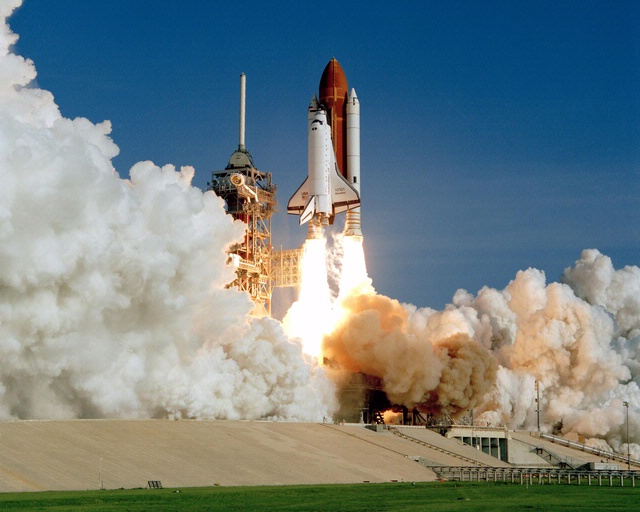
\includegraphics[scale=0.35]{gambar/roketluarangkasa.jpg}

  % Ubah dengan keterangan gambar yang diinginkan
  \caption{Peluncuran roket luar angkasa \emph{Discovery} \parencite{roketluarangkasa}.}
  \label{fig:roketluarangkasa}
\end{figure}

Roket luar angkasa merupakan \lipsum[1]

\emph{Discovery}, Gambar \ref{fig:roketluarangkasa}, merupakan \lipsum[2]

\section{Gravitasi}
\label{sec:gravitasi}

Gravitasi merupakan \lipsum[1]

\subsection{Hukum Newton}
\label{subsec:hukumnewton}

Newton \parencite{newton1687} pernah merumuskan bahwa \lipsum[1]
Kemudian menjadi persamaan seperti pada persamaan \ref{eq:hukumpertamanewton}.

% Contoh pembuatan persamaan
\begin{equation}
  \label{eq:hukumpertamanewton}
  \sum \mathbf{F} = 0\; \Leftrightarrow\; \frac{\mathrm{d} \mathbf{v} }{\mathrm{d}t} = 0.
\end{equation}

\subsection{Anti Gravitasi}
\label{subsec:antigravitasi}

Anti gravitasi merupakan \lipsum[1]

\cleardoublepage

% Bab 3 desain dan implementasi
\chapter{DESAIN DAN IMPLEMENTASI}
\label{chap:desainimplementasi}

% Ubah bagian-bagian berikut dengan isi dari desain dan implementasi

Penelitian ini dilaksanakan sesuai \lipsum[1][1-5]

\section{Deskripsi Sistem}
\label{sec:deskripsisistem}

Sistem akan dibuat dengan \lipsum[1-2]

\section{Implementasi Alat
  \label{sec:implementasi alat}}

Alat diimplementasikan dengan \lipsum[1]

% Contoh pembuatan potongan kode
\begin{lstlisting}[
  language=C++,
  caption={Program halo dunia.},
  label={lst:halodunia}
]
#include <iostream>

int main() {
    std::cout << "Halo Dunia!";
    return 0;
}
\end{lstlisting}

\lipsum[2-3]

% Contoh input potongan kode dari file
\lstinputlisting[
  language=Python,
  caption={Program perhitungan bilangan prima.},
  label={lst:bilanganprima}
]{program/bilangan-prima.py}

\lipsum[4]

\cleardoublepage

% Bab 4 pengujian dan analisis
\chapter{PENGUJIAN DAN ANALISIS}
\label{chap:pengujiananalisis}

% Ubah bagian-bagian berikut dengan isi dari pengujian dan analisis

Pada penelitian ini dipaparkan \lipsum[1][1-5]

\section{Skenario Pengujian}
\label{sec:skenariopengujian}

Pengujian dilakukan dengan \lipsum[1-2]

\section{Evaluasi Pengujian}
\label{sec:analisispengujian}

Dari pengujian yang \lipsum[1]

% Contoh pembuatan tabel
\begin{longtable}{|c|c|c|}
  \caption{Hasil Pengukuran Energi dan Kecepatan}
  \label{tb:EnergiKecepatan}                                   \\
  \hline
  \rowcolor[HTML]{C0C0C0}
  \textbf{Energi} & \textbf{Jarak Tempuh} & \textbf{Kecepatan} \\
  \hline
  10 J            & 1000 M                & 200 M/s            \\
  20 J            & 2000 M                & 400 M/s            \\
  30 J            & 4000 M                & 800 M/s            \\
  40 J            & 8000 M                & 1600 M/s           \\
  \hline
\end{longtable}

\lipsum[2-4]

\cleardoublepage

% Bab 5 penutup
\chapter{PENUTUP}
\label{chap:penutup}

% Ubah bagian-bagian berikut dengan isi dari penutup

\section{Kesimpulan}
\label{sec:kesimpulan}

Berdasarkan hasil pengujian yang \lipsum[1][1-3] sebagai berikut:

\begin{enumerate}[nolistsep]

  \item Pembuatan \lipsum[2][1-3]

  \item \lipsum[2][4-6]

  \item \lipsum[2][7-10]

\end{enumerate}

\section{Saran}
\label{chap:saran}

Untuk pengembangan lebih lanjut pada \lipsum[1][1-3] antara lain:

\begin{enumerate}[nolistsep]

  \item Memperbaiki \lipsum[2][1-3]

  \item \lipsum[2][4-6]

  \item \lipsum[2][7-10]

\end{enumerate}

\cleardoublepage

\chapter*{DAFTAR PUSTAKA}
\addcontentsline{toc}{chapter}{DAFTAR PUSTAKA}
\renewcommand\refname{}
\vspace{2ex}
\renewcommand{\bibname}{}
\begingroup
\def\chapter*#1{}
\printbibliography
\endgroup
\cleardoublepage

% Biografi penulis
\begin{center}
  \Large
  \textbf{BIOGRAFI PENULIS}
\end{center}

\addcontentsline{toc}{chapter}{BIOGRAFI PENULIS}

\vspace{2ex}

\begin{wrapfigure}{L}{0.3\textwidth}
  \centering
  \vspace{-3ex}
  % Ubah file gambar berikut dengan file foto dari mahasiswa
  
\includegraphics[width=0.3\textwidth]{gambar/elon.jpg}
  \vspace{-4ex}
\end{wrapfigure}

% Ubah kalimat berikut dengan biografi dari mahasiswa
\name{}, lahir pada \lipsum[1]

\lipsum[2]

\cleardoublepage

\end{document}
